\documentclass[12pt]{article}

\usepackage{algpseudocode}
\usepackage{algorithm}
\usepackage{amsmath}
\usepackage{amsfonts}
\usepackage{float}
\usepackage{fancyhdr}
\usepackage{graphicx}
\usepackage[colorlinks=true,linkcolor=blue, citecolor=red]{hyperref}
\usepackage{url}
\usepackage[top=1in, left=.5in, right=.5in]{geometry}
\usepackage[utf8]{vietnam}
\usepackage{biblatex}
\usepackage{listings}

\graphicspath{{img/}}
\addbibresource{main.bib}
\setlength{\headheight}{29.43912pt}
\addtolength{\topmargin}{-17.43912pt}

\pagestyle{fancy}
\lhead{
	Báo cáo đồ án 01
}
\rhead{
    Trường Đại học Khoa học Tự nhiên - ĐHQG HCM\\
    CSC15005 - Nhập môn mã hóa - mật mã
}
\lfoot{\LaTeX\ by \href{https://github.com/trhgquan}{Trần Hoàng Quân}}

\title{
	Báo cáo Đồ án 01\\ 
	Hệ thống lưu trữ file an toàn (mức độ sơ khai)
}
\author{Nhóm: navi no1}

\begin{document}
\maketitle
\tableofcontents
\pagebreak

\section{Thông tin nhóm}
\begin{center}
\begin{tabular}{ | c | c | c | } 
    \hline
    MSSV & Họ và tên\\
    \hline
    19120064 & Nguyễn Hồ Hoàng Duy\\
    \hline
    19120179 & Võ Trương Trung Chánh\\
    \hline
    19120266 & Nguyễn Hoàng Anh Kiệt\\
    \hline
    19120338 & Trần Hoàng Quân\\
    \hline
\end{tabular}
\end{center}

\section{Thông tin kỹ thuật}
Đồ án được thực hiện trên ngôn ngữ Python, sử dụng một số thư viện hỗ trợ sau:
\begin{itemize}
    \item Flask Framework và Flask RESTful: xây dựng RESTful API với Flask webframework.
    \item Thư viện AES mã nguồn mở của PyCryptodome.
    \item Thư viện secrets: tạo ngẫu nhiên các chuỗi với độ dài xác định.
    \item Thư viện hashlib : hỗ trợ các thuật toán SHA256, MD5, ..
    \item Thư viện PIL, OpenCV: chuyển đổi định dạng ảnh và thao tác với ảnh.
\end{itemize}
Các yêu cầu kĩ thuật để cài đặt và chạy thử sẽ được miêu tả rõ hơn ở phần \ref{caidatchaythu_subsec} 

\section{Giới thiệu về Protocol}
\subsection{Đăng ký}
Quá trình đăng ký được miêu tả như sau:
\begin{enumerate}
\item User nhập tên của mình vào client.
\item Client tiến hành tạo ngẫu nhiên cặp khóa RSA $e, d$.
\item User chọn cặp khóa tùy ý, rồi submit lên server để đăng ký.
\end{enumerate}
Ưu điểm của cách làm này là đảm bảo được user là người sở hữu khóa $e$. Sau đó user tiến hành ghi nhớ ID và khóa $d$, đây sẽ lần lượt là ID đăng nhập và mật khẩu đăng nhập cho tài khoản.

\subsection{Đăng nhập}
Quá trình đăng nhập được miêu tả như sau:
\begin{enumerate}
\item User tiến hành nhập ID và mật khẩu $d$.
\item Client sẽ gửi yêu cầu đăng nhập tới server, kèm theo ID của user.
\item Server sẽ tạo một token ngẫu nhiên\footnote{bằng \texttt{secrets.token\_hex}} và lưu 1 bản sao trong database, sau đó encrypt token bằng public key $e$ của user và gửi trả token đã được encrypt về client.
\item Client sẽ nhận token và dùng khóa $d$ để giải mã token bằng thuật toán RSA, sau đó gửi token ngược lại server.
\item Nếu token gửi lên giống với token trong database, server sẽ cấp cho user một API token sử dụng trong suốt session của mình.
\end{enumerate}
Cần lưu ý là khóa bí mật $d$ không bao giờ được gửi đi khỏi client. Như vậy, giả sử người dùng có bị lộ khóa công khai $e$ thì cũng không ảnh hưởng đến quá trình đăng nhập; ngược lại, giả sử khóa $e$ bị kẻ tấn công thay thế từ pha đăng ký, khi đó tài khoản sẽ không thể đăng nhập từ lần đầu tiên - hạn chế khả năng bị đánh tráo khóa công khai.

\subsection{Upload, Download \& Chia sẻ ảnh}
\begin{figure}[H]
\centering
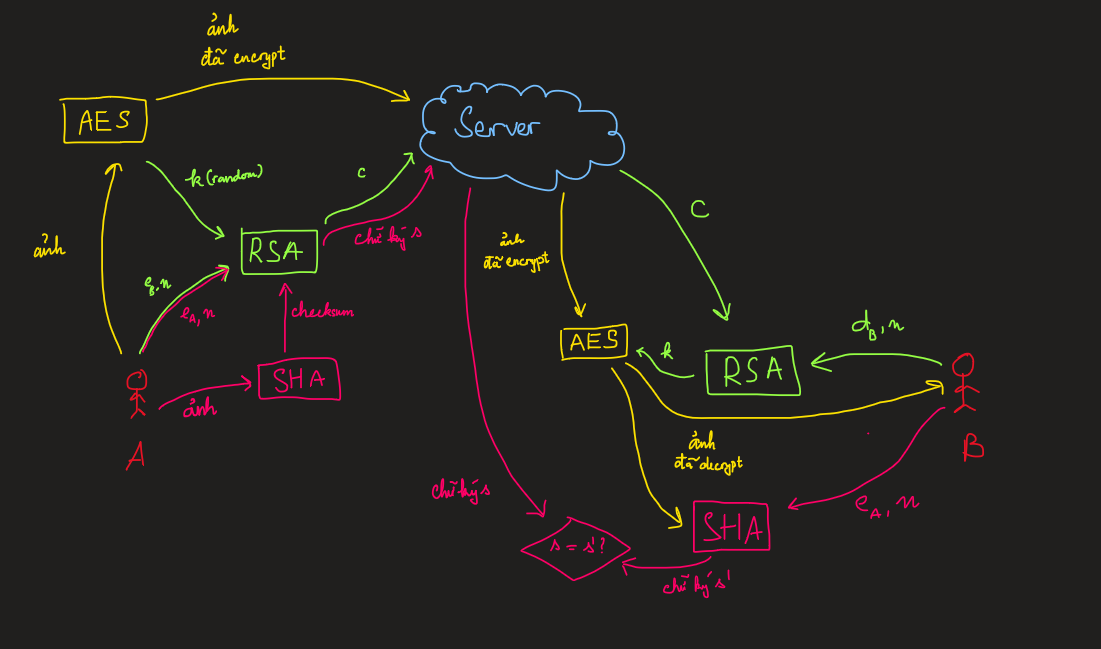
\includegraphics[scale=0.75]{upload-protocol.png}
\caption{Ảnh minh họa các giao thức upload ảnh và download ảnh}
\end{figure}

\subsubsection{Upload ảnh}
Giao thức upload ảnh được miêu tả như sau: Giả sử $A$ là người upload ảnh \texttt{a.jpg}, $A$ có khóa công khai $e_A$
\begin{enumerate}
\item Client sinh khóa ngẫu nhiên $k$.
\item Client dùng khóa $k$ mã hóa ảnh \texttt{a.jpg} bằng thuật toán AES.
\item Client dùng khóa công khai $e_A$ mã hóa $k$ thành $c$.
\item Client gửi ảnh đã mã hóa và $c$ lên server.
\end{enumerate}
Trong giao thức này có một bước nữa: tạo checksum để kiểm tra tính  toàn vẹn của ảnh:
\begin{enumerate}
\item Client hash ảnh bằng thuật toán SHA256 thành một chuỗi checksum $h$.
\item Client tiến hành mã hóa $h$ bằng thuật toán RSA với khóa công khai $e_A$, tạo chữ ký $s$.
\item Client gửi chữ ký $s$ lên server.
\end{enumerate}

\subsubsection{Download ảnh}
Giao thức download ảnh được miêu tả như sau: giả sử $A$ có quyền download ảnh (được chia sẻ ảnh) và có khóa bí mật $d_A$; $B$ là người upload ảnh có khóa công khai là $e_B$; Ảnh được upload lên server có chữ ký $s$.
\begin{enumerate}
\item Client download ảnh đã được mã hóa từ server.
\item Client yêu cầu lấy khóa $c$ từ server.
\item Client dùng khóa bí mật $d_A$ để giải mã $c$ trở thành $k$ bằng thuật toán RSA.
\item Client dùng $k$ để giải mã ảnh đã được mã hóa.
\end{enumerate}
Giao thức này còn một bước, là kiểm tra checksum của ảnh:
\begin{enumerate}
\item Client băm ảnh vừa được giải mã bên trên bằng thuật toán SHA256, tạo chuỗi checksum $h$.
\item Client dùng khóa công khai $e_B$ của $B$ mã hóa $h$ thành chữ ký $s'$, sử dụng thuật toán RSA.
\item Client sau đó so sánh $s'$ với $s$, nếu 2 chuỗi này trùng khớp thì ảnh được download nguyên vẹn, giống với ảnh gốc mà $B$ đã upload.
\end{enumerate}

\subsubsection{Chia sẻ ảnh}
\begin{figure}[H]
\centering
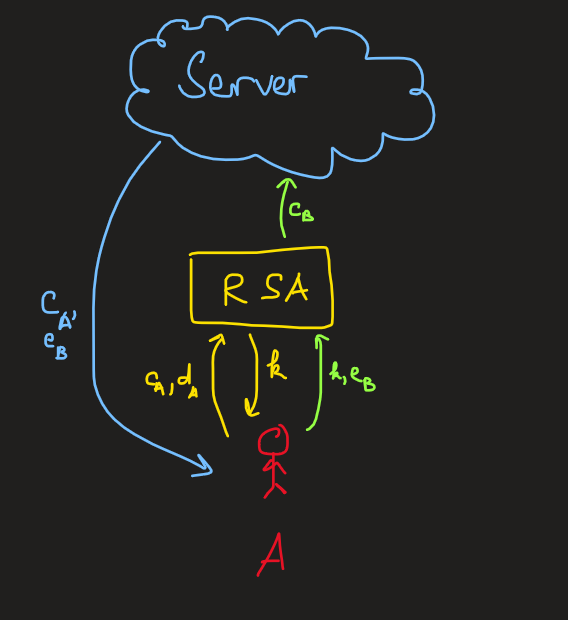
\includegraphics[]{sharing-protocol.png}
\caption{Ảnh minh họa giao thức chia sẻ ảnh}
\end{figure}

Giao thức chia sẻ ảnh được miêu tả như sau: giả sử $A$ \textbf{là chủ sở hữu của ảnh} muốn chia sẻ ảnh \texttt{x.jpg} cho $B$
\begin{itemize}
\item $A$ yêu cầu $c_A, e_B$ lần lượt là khóa mã ảnh \texttt{x.jpg} được mã hóa bởi $A$ và khóa công khai của $B$.
\item $A$ tiến hành giải mã khóa $c_A$ thành $k$ bằng khóa bí mật $d_A$ mình đang giữ, sử dụng thuật toán RSA.
\item $A$ mã hóa $k$ thành $c_B$ bằng khóa công khai $e_B$ của $B$, sau đó gửi $c_B$ trở lại server.
\end{itemize}
Khi đó $B$ chỉ cần yêu cầu download ảnh từ server và đã có khóa $c_B$ để giải mã.

\subsection{API}
Tài liệu API xem ở link này: \href{https://documenter.getpostman.com/view/18981203/UVRHiiVn}{https://documenter.getpostman.com/view/18981203/UVRHiiVn}

\section{Vận dụng}
\subsection{Các thuật toán sử dụng}
\subsubsection{RSA}
Nhóm cài đặt lại RSA protocol theo nội dung được giảng dạy trên lớp.:
\begin{enumerate}
\item Chọn $p, q$ là 2 số nguyên tố lớn.
\item Tính $n = pq, \phi = (p - 1)(q - 1)$
\item Chọn $d, e$ sao cho $e \equiv d^{-1} \pmod \phi$
\item Bản mã $c \equiv m^e \pmod n$
\item Bản rõ $m \equiv c^d \pmod n$
\end{enumerate}
Các phép nhân, phép mũ sử dụng thuật toán nhân nhanh và mũ nhanh theo modulo.
\subsubsection{Thuật toán Euclide mở rộng}
Dựa trên bổ đề Bézout: với hai số nguyên không âm $a$ và $b$, $g = (a, b)$ thì:
\begin{itemize}
\item Tồn tại hai số nguyên $x, y$ sao cho $ax + by = g$
\item $g$ là số nguyên nhỏ nhất có thể viết dưới dạng $ax + by$
\item Mỗi số $e$ có dạng $ax + by$ đều là bội của $d$.
\end{itemize}
Thuật toán nhận vào $a, b$, đưa ra $x, y; g = (a, b)$ sao cho $ax + by = g$
\begin{algorithm}[H]
\caption{Thuật toán Euclide mở rộng (Extended Euclidean Algorithm)}
\begin{algorithmic}
\Function{XEuclidean}{a, b}
\If{$a = 0$}
\Return{(b, 0, 1)}
\Else
\State $(g, y, x) \gets XEuclidean(b \% a, a)$

\State $\displaystyle x \gets x - \left\lfloor\frac{b}{a}\right\rfloor \times y$

\Return{$(g, x, y)$}
\EndIf
\EndFunction
\end{algorithmic}
\end{algorithm}

\subsubsection{Tìm modulo nghịch đảo}
Vẫn dựa trên bổ để Bézout bên trên: giả sử ta có $ax + by = g \iff ax \equiv g \pmod y$. Khi đó $x$ là modulo nghịch đảo của $a$ khi $g = 1$.

\begin{algorithm}
\caption{Thuật toán tìm modulo nghịch đảo}
\begin{algorithmic}
\Function{inverse\_modulo}{a, n}
\State $(g, x) \gets XEuclidean(a, n)$

\If{$g \neq 1$}
    \Return{`DnE`}
\Else 

\Return{x \% n}
\EndIf
\EndFunction
\end{algorithmic}
\end{algorithm}

\subsubsection{Thuật toán sinh khóa RSA ngẫu nhiên}
Sinh khóa RSA sử dụng 2 thuật toán chính:
\begin{itemize}
    \item Sinh số nguyên tố lớn (sử dụng để tạo $p, q$)
    \item Kiểm tra số nguyên tố
\end{itemize}
Để sinh $d, e$ ta chỉ cần sinh một số ngẫu nhiên trong $(1, \phi]$ và tìm khả nghịch của số đó trong $\phi$.

\subsubsection{AES - mã hóa và giải mã file ảnh}
\begin{figure}[H]
\centering
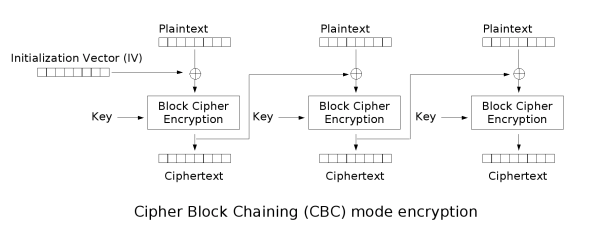
\includegraphics[]{Cbc_encryption.png}
\caption{Tóm tắt mode CBC.\cite{WikipediaEN:CBC} Thuật toán block encryption sử dụng ở đây là AES.}
\end{figure}

Nhóm sử dụng thuật toán AES trong thư viện PyCryptodome với mode CBC. Với cách làm này ảnh vẫn sẽ giữ nguyên format nhưng nội dung được làm nhiễu. Quá trình mã hóa:
\begin{itemize}
\item Vì ta muốn mã hóa nhiều format ảnh khác nhau, nhóm ưu tiên chuyển các ảnh về định dạng PNG bằng thư viện PIL. Việc chuyển format về dạng PNG giúp đảm bảo chất lượng của ảnh.
\item Khởi tạo khóa $k$ là một chuỗi ngẫu nhiên, ở đây nhóm chọn độ dài là 16 bytes. Khởi tạo block $\text{iv} = 0000000000000000$ cũng có cùng độ dài.
\item Tiến hành thêm padding cho file để file có kích thước là bội của 16. Byte cuối cùng của phần padding sẽ lưu số lượng dòng padding đã thêm. Chú ý là nếu file đã có kích thước là bội của 16, ta vẫn tiến hành thêm 16 bytes. Lúc này byte cuối cùng sẽ lưu số 16.\footnote{Nếu không thì trong quá trình giải mã, decryptor sẽ nhận "nhầm" byte cuối lưu 1 điểm ảnh RGB là số dòng cần xóa!}
\item Tiến hành mã hóa với AES và lưu vào file có định dạng PNG.
\end{itemize}
Với quá trình giải mã:
\begin{itemize}
\item Từ file và key ban đầu, dùng thuật toán AES để giải mã và cho vào một ma trận.
\item Phần tử cuối của ma trận lưu số dòng padding. Xóa các dòng padding đi.
\item Lưu ma trận trên vào file với định dạng gốc, sử dụng OpenCV.
\end{itemize}
Cách làm này được tham khảo từ câu trả lời trên StackOverflow của tác giả Rotem\cite{68046596}

\subsection{Cài đặt \& chạy thử}\label{caidatchaythu_subsec}
\subsubsection{Server}
Sử dụng Terminal (Linux) hoặc Command Line (Windows)
\begin{enumerate}
\item Tạo virtual environment cho server:
\\\\
Browse đến thư mục \texttt{server}, sau đó:
\begin{itemize}
\item Đối với Linux:
\begin{lstlisting}[language=bash]
python3 -m venv venv
\end{lstlisting}
\item Đối với Windows:
\begin{lstlisting}
python -m venv venv
\end{lstlisting}
\end{itemize}

\item Kích hoạt virtual environment
\begin{itemize}
\item Đối với Linux:
\begin{lstlisting}[language=bash]
. venv/bin/activate
\end{lstlisting}

\item Đối với Windows:
\begin{lstlisting}
venv\Scripts\activate
\end{lstlisting}
\end{itemize}

\item Cài các package cần thiết:
\begin{lstlisting}
pip install -r requirements.txt
\end{lstlisting}

\item Tạo mới database
\begin{itemize}
\item Đối với Linux:
\begin{lstlisting}[language=bash]
export FLASK_APP=serverside
export FLASK_ENV=development
flask init-db
\end{lstlisting}

\item Đối với Windows:
\begin{lstlisting}
set FLASK_APP=serverside
set FLASK_ENV=development
flask init-db
\end{lstlisting}
\end{itemize}

\item Chạy server
\begin{lstlisting}
flask run
\end{lstlisting}

\end{enumerate}

\subsubsection{Client}
\begin{enumerate}
\item Trong folder \texttt{client}, chạy câu lệnh sau để cài các package cần thiết:
\begin{lstlisting}[language=bash]
pip install -r requirements.txt
\end{lstlisting}

\item Chạy file \texttt{main.py} để khởi động client.
\begin{lstlisting}[language=bash]
python main.py
\end{lstlisting}
\end{enumerate}

\subsubsection{Hướng dẫn sử dụng}
Sau khi khởi động cả server và client, nhập IP của server và connection port để kết nối với server.
\\
Vì đây là một console application, chủ yếu người dùng sẽ nhập từ bàn phím để chọn các menu item / nhập liệu. 

\paragraph{Đăng kí}
\begin{itemize}
    \item Người dùng chọn menu Register new account.
    \item Người dùng nhập tên.
    \item Hệ thống sẽ random ra cặp khóa $e$ và $d$ ngẫu nhiên. Nếu đồng ý thì bấm \texttt{y}, ngược lại bấm \texttt{n} sẽ tạo khóa mới.
    \item Nếu chọn khóa xong, người dùng sẽ thấy hiển thị thông báo đăng kí thành công.
\end{itemize}

\paragraph{Đăng nhập}
\begin{itemize}
    \item Người dùng chọn menu Login.
    \item Người dùng nhập ID.
    \item Người dùng nhập khóa bí mật và nhấn Enter.
    \item Thông báo đăng nhập thành công, người dùng sẽ được chuyển hướng đến menu chính.
\end{itemize}

\begin{figure}[H]
\centering
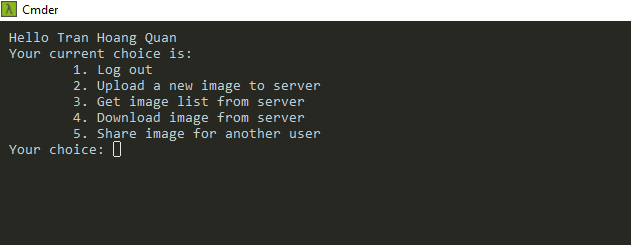
\includegraphics[]{main-menu.PNG}
\caption{Menu chính của client}
\end{figure}

\paragraph{Đăng xuất}

Trong menu chính, người dùng chọn Logout.

\paragraph{Upload ảnh}
\begin{itemize}
    \item Trong menu chính, người dùng chọn Upload a new image to server.
    \item Người dùng nhập đường dẫn đến file ảnh. Chú ý: Hệ thống chỉ hỗ trợ các extension \texttt{.png, .jpg/jpeg, .bmp}.
    \item Nhấn enter, người dùng đã upload ảnh thành công.
\end{itemize}

\begin{figure}[H]
\centering
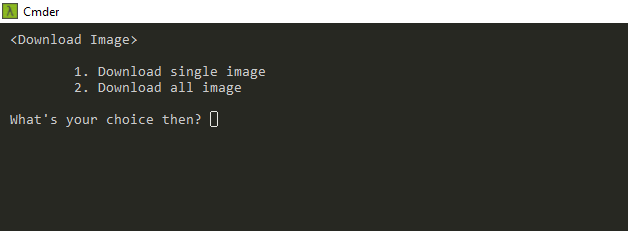
\includegraphics[]{download-menu.PNG}
\caption{Menu download}
\end{figure}

\paragraph{Download ảnh}

\begin{itemize}
    \item Trong menu chính, người dùng chọn Download image from server.
    \item Có 2 lựa chọn: download tất cả hoặc download 1 ảnh.
    \item Nếu download tất cả: hệ thống sẽ download tất cả những ảnh bạn đã upload / được chia sẻ.
    \item Nếu download 1 ảnh: nhập ID ảnh và download.
\end{itemize}

\begin{figure}[h]
\centering
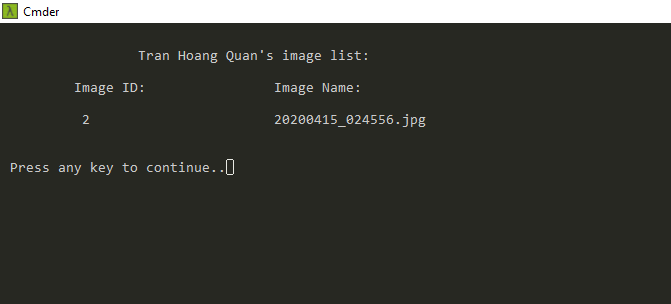
\includegraphics[]{list-image.PNG}
\caption{Danh sách ảnh của một User}
\end{figure}

\paragraph{Xem danh sách ảnh}

\begin{itemize}
    \item Trong menu chính, người dùng chọn Get image list from server.
    \item Tất cả các ảnh của user (upload, được share) sẽ được liệt kê ở đây (ID - tên ảnh)
\end{itemize}

\paragraph{Chia sẻ ảnh}

\begin{itemize}
    \item Trong menu chính, người dùng chọn Share image for another user.
    \item Người dùng nhập ID người cần share, ảnh cần share. Chú ý: người dùng phải là chủ (người upload) ảnh mới có thể share ảnh.
\end{itemize}

Chi tiết hướng dẫn sử dụng, mời bạn xem Demo.

\subsection{Demo}
Video demo quá trình cài đặt \& chạy thử ở link này.
\href{https://youtu.be/vQ0MhBgJ23A}{https://youtu.be/vQ0MhBgJ23A}

\section{Kết luận}
\subsection{Ưu điểm:}
\begin{itemize}
    \item Hệ thống có thể chia sẻ hình ảnh một cách bảo mật, không làm lộ thông tin cho bên thứ 3.
    \item File được lưu trữ nguyên vẹn, không bị tổn hại.
    \item Hệ thống đảm bảo chỉ những user có quyền (được chia sẻ) mới có thể xem ảnh; user có quyền (chủ sở hữu) mới có thể chia sẻ ảnh.
\end{itemize}
\subsection{Nhược điểm}
Vì đây là hệ thống ở mức độ sơ khai và không có hệ thống bảo mật nào là an toàn tuyệt đối, nên còn nhiều khuyết điểm cần chỉ rõ:
\begin{itemize}
    \item Hệ thống vẫn có thể làm lộ access\_token qua quá trình truyền tải nếu không có SSL encryption.
    \item Vì hệ thống chỉ hỗ trợ đăng nhập bằng khóa bí mật $d$, nên user chưa thể thay đổi password.
    \item Hệ thống chưa hỗ trợ tính năng xóa ảnh.
    \item Nếu nhiều user sử dụng cùng 1 máy thì rất dễ lộ folder Download. Hiện tại hệ thống chỉ hỗ trợ 1 user / máy.
\end{itemize}

\subsection{Cải tiến}
\begin{itemize}
    \item Có thể thay thế CBC mode bằng một số mode khác phức tạp hơn để đảm bảo độ an toàn cho ảnh đã encrypt.
    \item Có thể tăng độ dài key RSA và AES để đảm bảo an toàn.
\end{itemize}

\pagebreak
\printbibliography
\end{document}